\documentclass[1p]{elsarticle_modified}
%\bibliographystyle{elsarticle-num}

%\usepackage[colorlinks]{hyperref}
%\usepackage{abbrmath_seonhwa} %\Abb, \Ascr, \Acal ,\Abf, \Afrak
\usepackage{amsfonts}
\usepackage{amssymb}
\usepackage{amsmath}
\usepackage{amsthm}
\usepackage{scalefnt}
\usepackage{amsbsy}
\usepackage{kotex}
\usepackage{caption}
\usepackage{subfig}
\usepackage{color}
\usepackage{graphicx}
\usepackage{xcolor} %% white, black, red, green, blue, cyan, magenta, yellow
\usepackage{float}
\usepackage{setspace}
\usepackage{hyperref}

\usepackage{tikz}
\usetikzlibrary{arrows}

\usepackage{multirow}
\usepackage{array} % fixed length table
\usepackage{hhline}

%%%%%%%%%%%%%%%%%%%%%
\makeatletter
\renewcommand*\env@matrix[1][\arraystretch]{%
	\edef\arraystretch{#1}%
	\hskip -\arraycolsep
	\let\@ifnextchar\new@ifnextchar
	\array{*\c@MaxMatrixCols c}}
\makeatother %https://tex.stackexchange.com/questions/14071/how-can-i-increase-the-line-spacing-in-a-matrix
%%%%%%%%%%%%%%%

\usepackage[normalem]{ulem}

\newcommand{\msout}[1]{\ifmmode\text{\sout{\ensuremath{#1}}}\else\sout{#1}\fi}
%SOURCE: \msout is \stkout macro in https://tex.stackexchange.com/questions/20609/strikeout-in-math-mode

\newcommand{\cancel}[1]{
	\ifmmode
	{\color{red}\msout{#1}}
	\else
	{\color{red}\sout{#1}}
	\fi
}

\newcommand{\add}[1]{
	{\color{blue}\uwave{#1}}
}

\newcommand{\replace}[2]{
	\ifmmode
	{\color{red}\msout{#1}}{\color{blue}\uwave{#2}}
	\else
	{\color{red}\sout{#1}}{\color{blue}\uwave{#2}}
	\fi
}

\newcommand{\Sol}{\mathcal{S}} %segment
\newcommand{\D}{D} %diagram
\newcommand{\A}{\mathcal{A}} %arc


%%%%%%%%%%%%%%%%%%%%%%%%%%%%%5 test

\def\sl{\operatorname{\textup{SL}}(2,\Cbb)}
\def\psl{\operatorname{\textup{PSL}}(2,\Cbb)}
\def\quan{\mkern 1mu \triangleright \mkern 1mu}

\theoremstyle{definition}
\newtheorem{thm}{Theorem}[section]
\newtheorem{prop}[thm]{Proposition}
\newtheorem{lem}[thm]{Lemma}
\newtheorem{ques}[thm]{Question}
\newtheorem{cor}[thm]{Corollary}
\newtheorem{defn}[thm]{Definition}
\newtheorem{exam}[thm]{Example}
\newtheorem{rmk}[thm]{Remark}
\newtheorem{alg}[thm]{Algorithm}

\newcommand{\I}{\sqrt{-1}}
\begin{document}

%\begin{frontmatter}
%
%\title{Boundary parabolic representations of knots up to 8 crossings}
%
%%% Group authors per affiliation:
%\author{Yunhi Cho} 
%\address{Department of Mathematics, University of Seoul, Seoul, Korea}
%\ead{yhcho@uos.ac.kr}
%
%
%\author{Seonhwa Kim} %\fnref{s_kim}}
%\address{Center for Geometry and Physics, Institute for Basic Science, Pohang, 37673, Korea}
%\ead{ryeona17@ibs.re.kr}
%
%\author{Hyuk Kim}
%\address{Department of Mathematical Sciences, Seoul National University, Seoul 08826, Korea}
%\ead{hyukkim@snu.ac.kr}
%
%\author{Seokbeom Yoon}
%\address{Department of Mathematical Sciences, Seoul National University, Seoul, 08826,  Korea}
%\ead{sbyoon15@snu.ac.kr}
%
%\begin{abstract}
%We find all boundary parabolic representation of knots up to 8 crossings.
%
%\end{abstract}
%\begin{keyword}
%    \MSC[2010] 57M25 
%\end{keyword}
%
%\end{frontmatter}

%\linenumbers
%\tableofcontents
%
\newcommand\colored[1]{\textcolor{white}{\rule[-0.35ex]{0.8em}{1.4ex}}\kern-0.8em\color{red} #1}%
%\newcommand\colored[1]{\textcolor{white}{ #1}\kern-2.17ex	\textcolor{white}{ #1}\kern-1.81ex	\textcolor{white}{ #1}\kern-2.15ex\color{red}#1	}

{\Large $\underline{12a_{0790}~(K12a_{0790})}$}

\setlength{\tabcolsep}{10pt}
\renewcommand{\arraystretch}{1.6}
\vspace{1cm}\begin{tabular}{m{100pt}>{\centering\arraybackslash}m{274pt}}
\multirow{5}{120pt}{
	\centering
	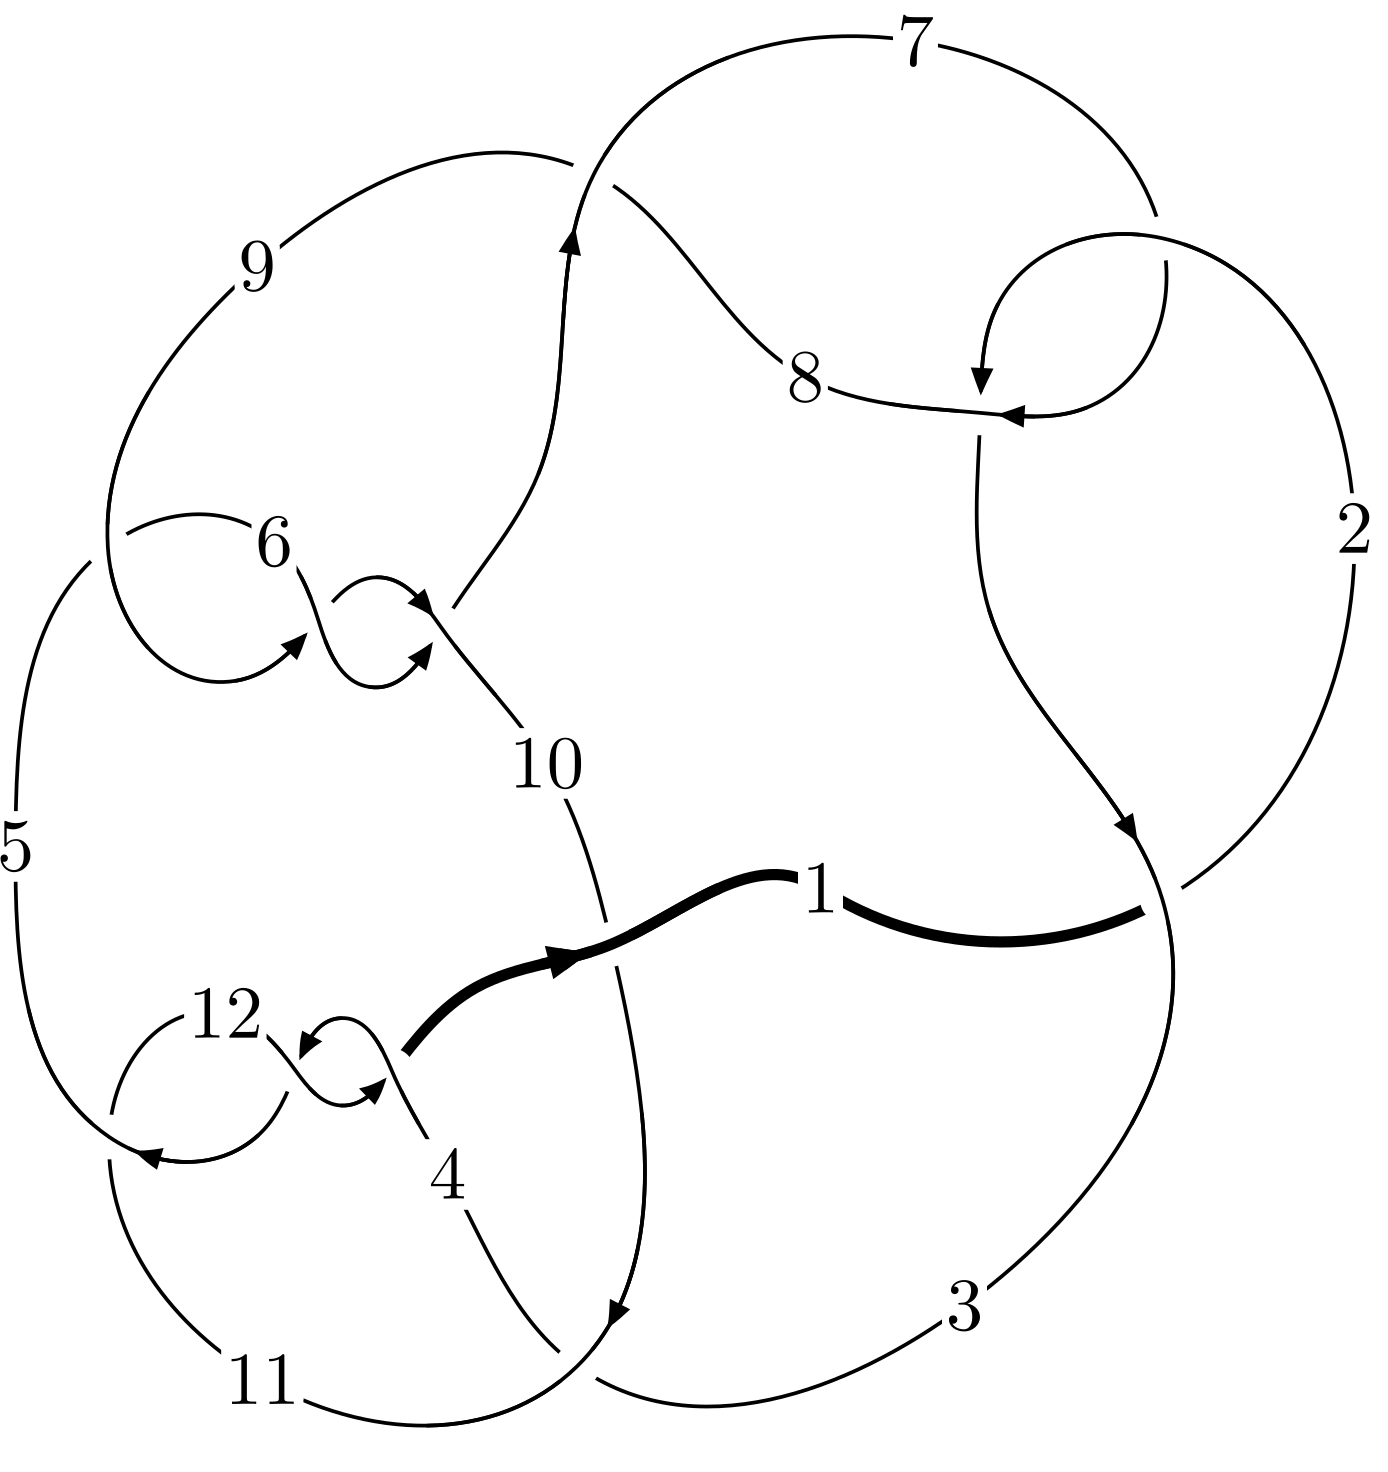
\includegraphics[width=112pt]{../../../GIT/diagram.site/Diagrams/png/1591_12a_0790.png}\\
\ \ \ A knot diagram\footnotemark}&
\allowdisplaybreaks
\textbf{Linearized knot diagam} \\
\cline{2-2}
 &
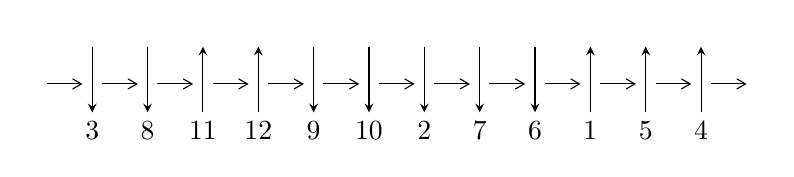
\begin{tikzpicture}[x=20pt, y=17pt]
	% nodes
	\node (C0) at (0, 0) {};
	\node (C1) at (1, 0) {};
	\node (C1U) at (1, +1) {};
	\node (C1D) at (1, -1) {3};

	\node (C2) at (2, 0) {};
	\node (C2U) at (2, +1) {};
	\node (C2D) at (2, -1) {8};

	\node (C3) at (3, 0) {};
	\node (C3U) at (3, +1) {};
	\node (C3D) at (3, -1) {11};

	\node (C4) at (4, 0) {};
	\node (C4U) at (4, +1) {};
	\node (C4D) at (4, -1) {12};

	\node (C5) at (5, 0) {};
	\node (C5U) at (5, +1) {};
	\node (C5D) at (5, -1) {9};

	\node (C6) at (6, 0) {};
	\node (C6U) at (6, +1) {};
	\node (C6D) at (6, -1) {10};

	\node (C7) at (7, 0) {};
	\node (C7U) at (7, +1) {};
	\node (C7D) at (7, -1) {2};

	\node (C8) at (8, 0) {};
	\node (C8U) at (8, +1) {};
	\node (C8D) at (8, -1) {7};

	\node (C9) at (9, 0) {};
	\node (C9U) at (9, +1) {};
	\node (C9D) at (9, -1) {6};

	\node (C10) at (10, 0) {};
	\node (C10U) at (10, +1) {};
	\node (C10D) at (10, -1) {1};

	\node (C11) at (11, 0) {};
	\node (C11U) at (11, +1) {};
	\node (C11D) at (11, -1) {5};

	\node (C12) at (12, 0) {};
	\node (C12U) at (12, +1) {};
	\node (C12D) at (12, -1) {4};
	\node (C13) at (13, 0) {};

	% arrows
	\draw[->,>={angle 60}]
	(C0) edge (C1) (C1) edge (C2) (C2) edge (C3) (C3) edge (C4) (C4) edge (C5) (C5) edge (C6) (C6) edge (C7) (C7) edge (C8) (C8) edge (C9) (C9) edge (C10) (C10) edge (C11) (C11) edge (C12) (C12) edge (C13) ;	\draw[->,>=stealth]
	(C1U) edge (C1D) (C2U) edge (C2D) (C3D) edge (C3U) (C4D) edge (C4U) (C5U) edge (C5D) (C6U) edge (C6D) (C7U) edge (C7D) (C8U) edge (C8D) (C9U) edge (C9D) (C10D) edge (C10U) (C11D) edge (C11U) (C12D) edge (C12U) ;
	\end{tikzpicture} \\
\hhline{~~} \\& 
\textbf{Solving Sequence} \\ \cline{2-2} 
 &
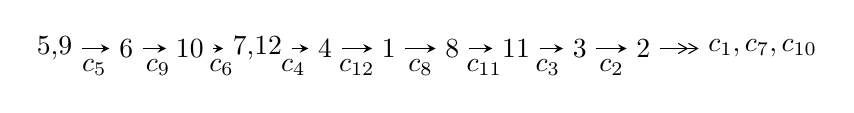
\begin{tikzpicture}[x=23pt, y=7pt]
	% node
	\node (A0) at (-1/8, 0) {5,9};
	\node (A1) at (1, 0) {6};
	\node (A2) at (2, 0) {10};
	\node (A3) at (49/16, 0) {7,12};
	\node (A4) at (33/8, 0) {4};
	\node (A5) at (41/8, 0) {1};
	\node (A6) at (49/8, 0) {8};
	\node (A7) at (57/8, 0) {11};
	\node (A8) at (65/8, 0) {3};
	\node (A9) at (73/8, 0) {2};
	\node (C1) at (1/2, -1) {$c_{5}$};
	\node (C2) at (3/2, -1) {$c_{9}$};
	\node (C3) at (5/2, -1) {$c_{6}$};
	\node (C4) at (29/8, -1) {$c_{4}$};
	\node (C5) at (37/8, -1) {$c_{12}$};
	\node (C6) at (45/8, -1) {$c_{8}$};
	\node (C7) at (53/8, -1) {$c_{11}$};
	\node (C8) at (61/8, -1) {$c_{3}$};
	\node (C9) at (69/8, -1) {$c_{2}$};
	\node (A10) at (11, 0) {$c_{1},c_{7},c_{10}$};

	% edge
	\draw[->,>=stealth]	
	(A0) edge (A1) (A1) edge (A2) (A2) edge (A3) (A3) edge (A4) (A4) edge (A5) (A5) edge (A6) (A6) edge (A7) (A7) edge (A8) (A8) edge (A9) ;
	\draw[->>,>={angle 60}]	
	(A9) edge (A10);
\end{tikzpicture} \\ 

\end{tabular} \\

\footnotetext{
The image of knot diagram is generated by the software ``\textbf{Draw programme}" developed by Andrew Bartholomew(\url{http://www.layer8.co.uk/maths/draw/index.htm\#Running-draw}), where we modified some parts for our purpose(\url{https://github.com/CATsTAILs/LinksPainter}).
}\phantom \\ \newline 
\centering \textbf{Ideals for irreducible components\footnotemark of $X_{\text{par}}$} 
 
\begin{align*}
I^u_{1}&=\langle 
- u^{73}+3 u^{72}+\cdots+4 b-1,\;- u^{73}+3 u^{72}+\cdots+4 a+3,\;u^{74}-4 u^{73}+\cdots+u-1\rangle \\
I^u_{2}&=\langle 
b- a-1,\;a^3+2 a^2+3 a+1,\;u-1\rangle \\
\\
\end{align*}
\raggedright * 2 irreducible components of $\dim_{\mathbb{C}}=0$, with total 77 representations.\\
\footnotetext{All coefficients of polynomials are rational numbers. But the coefficients are sometimes approximated in decimal forms when there is not enough margin.}
\newpage
\renewcommand{\arraystretch}{1}
\centering \section*{I. $I^u_{1}= \langle - u^{73}+3 u^{72}+\cdots+4 b-1,\;- u^{73}+3 u^{72}+\cdots+4 a+3,\;u^{74}-4 u^{73}+\cdots+u-1 \rangle$}
\flushleft \textbf{(i) Arc colorings}\\
\begin{tabular}{m{7pt} m{180pt} m{7pt} m{180pt} }
\flushright $a_{5}=$&$\begin{pmatrix}1\\0\end{pmatrix}$ \\
\flushright $a_{9}=$&$\begin{pmatrix}0\\u\end{pmatrix}$ \\
\flushright $a_{6}=$&$\begin{pmatrix}1\\u^2\end{pmatrix}$ \\
\flushright $a_{10}=$&$\begin{pmatrix}- u\\- u^3+u\end{pmatrix}$ \\
\flushright $a_{7}=$&$\begin{pmatrix}- u^2+1\\- u^4+2 u^2\end{pmatrix}$ \\
\flushright $a_{12}=$&$\begin{pmatrix}\frac{1}{4} u^{73}-\frac{3}{4} u^{72}+\cdots-6 u-\frac{3}{4}\\\frac{1}{4} u^{73}-\frac{3}{4} u^{72}+\cdots-\frac{15}{4} u^2+\frac{1}{4}\end{pmatrix}$ \\
\flushright $a_{4}=$&$\begin{pmatrix}\frac{17}{4} u^{73}-\frac{49}{4} u^{72}+\cdots-\frac{1}{2} u+\frac{19}{4}\\5 u^{73}-\frac{29}{2} u^{72}+\cdots-\frac{1}{2} u+\frac{9}{2}\end{pmatrix}$ \\
\flushright $a_{1}=$&$\begin{pmatrix}\frac{21}{2} u^{73}-\frac{57}{2} u^{72}+\cdots-7 u+\frac{15}{2}\\\frac{77}{4} u^{73}-\frac{213}{4} u^{72}+\cdots-\frac{5}{2} u+\frac{63}{4}\end{pmatrix}$ \\
\flushright $a_{8}=$&$\begin{pmatrix}u^5-2 u^3+u\\u^7-3 u^5+2 u^3+u\end{pmatrix}$ \\
\flushright $a_{11}=$&$\begin{pmatrix}- u^{18}+7 u^{16}+\cdots-6 u-1\\\frac{1}{4} u^{73}-\frac{3}{4} u^{72}+\cdots-\frac{15}{4} u^2+\frac{1}{4}\end{pmatrix}$ \\
\flushright $a_{3}=$&$\begin{pmatrix}-\frac{25}{2} u^{73}+\frac{67}{2} u^{72}+\cdots-2 u-\frac{19}{2}\\\frac{59}{4} u^{73}-\frac{163}{4} u^{72}+\cdots-\frac{5}{2} u+\frac{49}{4}\end{pmatrix}$ \\
\flushright $a_{2}=$&$\begin{pmatrix}-\frac{1}{2} u^{73}+\frac{5}{2} u^{72}+\cdots-5 u-\frac{3}{2}\\\frac{117}{4} u^{73}-\frac{325}{4} u^{72}+\cdots-\frac{9}{2} u+\frac{95}{4}\end{pmatrix}$\\&\end{tabular}
\flushleft \textbf{(ii) Obstruction class $= -1$}\\~\\
\flushleft \textbf{(iii) Cusp Shapes $= 63 u^{73}-\frac{343}{2} u^{72}+\cdots-\frac{3}{2} u+\frac{101}{2}$}\\~\\
\newpage\renewcommand{\arraystretch}{1}
\flushleft \textbf{(iv) u-Polynomials at the component}\newline \\
\begin{tabular}{m{50pt}|m{274pt}}
Crossings & \hspace{64pt}u-Polynomials at each crossing \\
\hline $$\begin{aligned}c_{1},c_{8}\end{aligned}$$&$\begin{aligned}
&u^{74}+21 u^{73}+\cdots+848 u+64
\end{aligned}$\\
\hline $$\begin{aligned}c_{2},c_{7}\end{aligned}$$&$\begin{aligned}
&u^{74}+u^{73}+\cdots+12 u+8
\end{aligned}$\\
\hline $$\begin{aligned}c_{3}\end{aligned}$$&$\begin{aligned}
&u^{74}-2 u^{73}+\cdots-60 u-9
\end{aligned}$\\
\hline $$\begin{aligned}c_{4},c_{11},c_{12}\end{aligned}$$&$\begin{aligned}
&u^{74}+2 u^{73}+\cdots-6 u-1
\end{aligned}$\\
\hline $$\begin{aligned}c_{5},c_{6},c_{9}\end{aligned}$$&$\begin{aligned}
&u^{74}-4 u^{73}+\cdots+u-1
\end{aligned}$\\
\hline $$\begin{aligned}c_{10}\end{aligned}$$&$\begin{aligned}
&u^{74}+18 u^{73}+\cdots+560 u+49
\end{aligned}$\\
\hline
\end{tabular}\\~\\
\newpage\renewcommand{\arraystretch}{1}
\flushleft \textbf{(v) Riley Polynomials at the component}\newline \\
\begin{tabular}{m{50pt}|m{274pt}}
Crossings & \hspace{64pt}Riley Polynomials at each crossing \\
\hline $$\begin{aligned}c_{1},c_{8}\end{aligned}$$&$\begin{aligned}
&y^{74}+59 y^{73}+\cdots-36096 y+4096
\end{aligned}$\\
\hline $$\begin{aligned}c_{2},c_{7}\end{aligned}$$&$\begin{aligned}
&y^{74}-21 y^{73}+\cdots-848 y+64
\end{aligned}$\\
\hline $$\begin{aligned}c_{3}\end{aligned}$$&$\begin{aligned}
&y^{74}-6 y^{73}+\cdots+162 y+81
\end{aligned}$\\
\hline $$\begin{aligned}c_{4},c_{11},c_{12}\end{aligned}$$&$\begin{aligned}
&y^{74}+66 y^{73}+\cdots-14 y+1
\end{aligned}$\\
\hline $$\begin{aligned}c_{5},c_{6},c_{9}\end{aligned}$$&$\begin{aligned}
&y^{74}-60 y^{73}+\cdots+17 y+1
\end{aligned}$\\
\hline $$\begin{aligned}c_{10}\end{aligned}$$&$\begin{aligned}
&y^{74}+6 y^{73}+\cdots+49882 y+2401
\end{aligned}$\\
\hline
\end{tabular}\\~\\
\newpage\flushleft \textbf{(vi) Complex Volumes and Cusp Shapes}
$$\begin{array}{c|c|c}  
\text{Solutions to }I^u_{1}& \I (\text{vol} + \sqrt{-1}CS) & \text{Cusp shape}\\
 \hline 
\begin{aligned}
u &= -0.982931 + 0.351670 I \\
a &= \phantom{-}1.29013 - 1.44788 I \\
b &= -0.114226 - 1.346610 I\end{aligned}
 & -5.40881 + 1.48488 I & \phantom{-0.000000 } 0 \\ \hline\begin{aligned}
u &= -0.982931 - 0.351670 I \\
a &= \phantom{-}1.29013 + 1.44788 I \\
b &= -0.114226 + 1.346610 I\end{aligned}
 & -5.40881 - 1.48488 I & \phantom{-0.000000 } 0 \\ \hline\begin{aligned}
u &= -0.114338 + 0.877618 I \\
a &= \phantom{-}1.79001 - 0.30234 I \\
b &= -0.29499 - 1.39816 I\end{aligned}
 & \phantom{-}0.40081 + 10.70940 I & \phantom{-0.000000 } 0 \\ \hline\begin{aligned}
u &= -0.114338 - 0.877618 I \\
a &= \phantom{-}1.79001 + 0.30234 I \\
b &= -0.29499 + 1.39816 I\end{aligned}
 & \phantom{-}0.40081 - 10.70940 I & \phantom{-0.000000 } 0 \\ \hline\begin{aligned}
u &= -0.096801 + 0.866328 I \\
a &= \phantom{-}1.151770 - 0.473352 I \\
b &= -0.736562 - 0.242206 I\end{aligned}
 & \phantom{-}5.61875 + 6.96802 I & \phantom{-0.000000 } 0. - 6.74295 I \\ \hline\begin{aligned}
u &= -0.096801 - 0.866328 I \\
a &= \phantom{-}1.151770 + 0.473352 I \\
b &= -0.736562 + 0.242206 I\end{aligned}
 & \phantom{-}5.61875 - 6.96802 I & \phantom{-0.000000 -}0. + 6.74295 I \\ \hline\begin{aligned}
u &= -0.841922\phantom{ +0.000000I} \\
a &= \phantom{-}0.589364\phantom{ +0.000000I} \\
b &= -0.325299\phantom{ +0.000000I}\end{aligned}
 & -1.16434\phantom{ +0.000000I} & -11.0700\phantom{ +0.000000I} \\ \hline\begin{aligned}
u &= -0.071633 + 0.837460 I \\
a &= \phantom{-}0.325108 - 0.396010 I \\
b &= -0.289957 + 0.808580 I\end{aligned}
 & \phantom{-}3.72265 + 3.07550 I & \phantom{-0.000000 } 0. - 1.96212 I \\ \hline\begin{aligned}
u &= -0.071633 - 0.837460 I \\
a &= \phantom{-}0.325108 + 0.396010 I \\
b &= -0.289957 - 0.808580 I\end{aligned}
 & \phantom{-}3.72265 - 3.07550 I & \phantom{-0.000000 -}0. + 1.96212 I \\ \hline\begin{aligned}
u &= -0.032962 + 0.823375 I \\
a &= -0.347239 - 0.544285 I \\
b &= \phantom{-}0.256055 + 0.912970 I\end{aligned}
 & \phantom{-}3.87638 + 2.84826 I & \phantom{-0.000000 } 0. - 3.67608 I\\
 \hline 
 \end{array}$$\newpage$$\begin{array}{c|c|c}  
\text{Solutions to }I^u_{1}& \I (\text{vol} + \sqrt{-1}CS) & \text{Cusp shape}\\
 \hline 
\begin{aligned}
u &= -0.032962 - 0.823375 I \\
a &= -0.347239 + 0.544285 I \\
b &= \phantom{-}0.256055 - 0.912970 I\end{aligned}
 & \phantom{-}3.87638 - 2.84826 I & \phantom{-0.000000 -}0. + 3.67608 I \\ \hline\begin{aligned}
u &= \phantom{-}0.011012 + 0.810021 I \\
a &= -1.250280 - 0.486422 I \\
b &= \phantom{-}0.733701 - 0.206836 I\end{aligned}
 & \phantom{-}6.08567 - 0.95765 I & \phantom{-}3.69454 + 1.25612 I \\ \hline\begin{aligned}
u &= \phantom{-}0.011012 - 0.810021 I \\
a &= -1.250280 + 0.486422 I \\
b &= \phantom{-}0.733701 + 0.206836 I\end{aligned}
 & \phantom{-}6.08567 + 0.95765 I & \phantom{-}3.69454 - 1.25612 I \\ \hline\begin{aligned}
u &= \phantom{-}0.038683 + 0.799560 I \\
a &= -1.97178 - 0.13620 I \\
b &= \phantom{-}0.294669 - 1.379250 I\end{aligned}
 & \phantom{-}1.05738 - 4.68103 I & -0.94722 + 2.51196 I \\ \hline\begin{aligned}
u &= \phantom{-}0.038683 - 0.799560 I \\
a &= -1.97178 + 0.13620 I \\
b &= \phantom{-}0.294669 + 1.379250 I\end{aligned}
 & \phantom{-}1.05738 + 4.68103 I & -0.94722 - 2.51196 I \\ \hline\begin{aligned}
u &= -0.623280 + 0.490874 I \\
a &= -0.097681 + 1.280110 I \\
b &= -0.185972 + 1.388820 I\end{aligned}
 & -6.53161 - 2.00010 I & -10.45886 + 0. I\phantom{ +0.000000I} \\ \hline\begin{aligned}
u &= -0.623280 - 0.490874 I \\
a &= -0.097681 - 1.280110 I \\
b &= -0.185972 - 1.388820 I\end{aligned}
 & -6.53161 + 2.00010 I & -10.45886 + 0. I\phantom{ +0.000000I} \\ \hline\begin{aligned}
u &= -0.138267 + 0.766818 I \\
a &= -0.172017 + 0.580214 I \\
b &= -0.051081 + 1.397250 I\end{aligned}
 & -2.82199 + 2.49718 I & -4.67442 - 3.51648 I \\ \hline\begin{aligned}
u &= -0.138267 - 0.766818 I \\
a &= -0.172017 - 0.580214 I \\
b &= -0.051081 - 1.397250 I\end{aligned}
 & -2.82199 - 2.49718 I & -4.67442 + 3.51648 I \\ \hline\begin{aligned}
u &= \phantom{-}1.229430 + 0.060313 I \\
a &= -0.812751 - 0.979382 I \\
b &= \phantom{-}0.261875 - 1.235300 I\end{aligned}
 & -5.67724 - 3.54075 I & \phantom{-0.000000 } 0\\
 \hline 
 \end{array}$$\newpage$$\begin{array}{c|c|c}  
\text{Solutions to }I^u_{1}& \I (\text{vol} + \sqrt{-1}CS) & \text{Cusp shape}\\
 \hline 
\begin{aligned}
u &= \phantom{-}1.229430 - 0.060313 I \\
a &= -0.812751 + 0.979382 I \\
b &= \phantom{-}0.261875 + 1.235300 I\end{aligned}
 & -5.67724 + 3.54075 I & \phantom{-0.000000 } 0 \\ \hline\begin{aligned}
u &= \phantom{-}1.23207\phantom{ +0.000000I} \\
a &= -0.416426\phantom{ +0.000000I} \\
b &= \phantom{-}0.710023\phantom{ +0.000000I}\end{aligned}
 & -1.89563\phantom{ +0.000000I} & \phantom{-0.000000 } 0 \\ \hline\begin{aligned}
u &= -1.156710 + 0.449194 I \\
a &= \phantom{-}0.368328 + 1.040150 I \\
b &= -0.28561 + 1.38677 I\end{aligned}
 & -2.79362 - 5.97206 I & \phantom{-0.000000 } 0 \\ \hline\begin{aligned}
u &= -1.156710 - 0.449194 I \\
a &= \phantom{-}0.368328 - 1.040150 I \\
b &= -0.28561 - 1.38677 I\end{aligned}
 & -2.79362 + 5.97206 I & \phantom{-0.000000 } 0 \\ \hline\begin{aligned}
u &= -0.447414 + 0.610883 I \\
a &= \phantom{-}1.87368 - 1.20772 I \\
b &= -0.22452 - 1.39679 I\end{aligned}
 & -5.97032 + 6.07295 I & -8.10796 - 7.73862 I \\ \hline\begin{aligned}
u &= -0.447414 - 0.610883 I \\
a &= \phantom{-}1.87368 + 1.20772 I \\
b &= -0.22452 + 1.39679 I\end{aligned}
 & -5.97032 - 6.07295 I & -8.10796 + 7.73862 I \\ \hline\begin{aligned}
u &= -1.174400 + 0.427018 I \\
a &= \phantom{-}0.406561 - 0.005470 I \\
b &= -0.716781 + 0.220171 I\end{aligned}
 & \phantom{-}2.31230 - 2.33683 I & \phantom{-0.000000 } 0 \\ \hline\begin{aligned}
u &= -1.174400 - 0.427018 I \\
a &= \phantom{-}0.406561 + 0.005470 I \\
b &= -0.716781 - 0.220171 I\end{aligned}
 & \phantom{-}2.31230 + 2.33683 I & \phantom{-0.000000 } 0 \\ \hline\begin{aligned}
u &= -1.250100 + 0.050558 I \\
a &= \phantom{-}0.58611 + 1.34682 I \\
b &= \phantom{-}0.502125 + 0.290673 I\end{aligned}
 & -2.76802 + 1.42671 I & \phantom{-0.000000 } 0 \\ \hline\begin{aligned}
u &= -1.250100 - 0.050558 I \\
a &= \phantom{-}0.58611 - 1.34682 I \\
b &= \phantom{-}0.502125 - 0.290673 I\end{aligned}
 & -2.76802 - 1.42671 I & \phantom{-0.000000 } 0\\
 \hline 
 \end{array}$$\newpage$$\begin{array}{c|c|c}  
\text{Solutions to }I^u_{1}& \I (\text{vol} + \sqrt{-1}CS) & \text{Cusp shape}\\
 \hline 
\begin{aligned}
u &= -1.207660 + 0.387161 I \\
a &= \phantom{-}0.908549 - 0.496550 I \\
b &= -0.200242 - 0.878527 I\end{aligned}
 & \phantom{-}0.234639 + 1.326060 I & \phantom{-0.000000 } 0 \\ \hline\begin{aligned}
u &= -1.207660 - 0.387161 I \\
a &= \phantom{-}0.908549 + 0.496550 I \\
b &= -0.200242 + 0.878527 I\end{aligned}
 & \phantom{-}0.234639 - 1.326060 I & \phantom{-0.000000 } 0 \\ \hline\begin{aligned}
u &= -1.249840 + 0.252900 I \\
a &= \phantom{-}1.62462 - 2.52638 I \\
b &= \phantom{-}0.080915 - 1.377220 I\end{aligned}
 & -5.96096 + 0.85034 I & \phantom{-0.000000 } 0 \\ \hline\begin{aligned}
u &= -1.249840 - 0.252900 I \\
a &= \phantom{-}1.62462 + 2.52638 I \\
b &= \phantom{-}0.080915 + 1.377220 I\end{aligned}
 & -5.96096 - 0.85034 I & \phantom{-0.000000 } 0 \\ \hline\begin{aligned}
u &= \phantom{-}1.237920 + 0.345248 I \\
a &= -0.454616 + 1.014780 I \\
b &= \phantom{-}0.303590 + 1.360390 I\end{aligned}
 & -2.63807 + 0.55572 I & \phantom{-0.000000 } 0 \\ \hline\begin{aligned}
u &= \phantom{-}1.237920 - 0.345248 I \\
a &= -0.454616 - 1.014780 I \\
b &= \phantom{-}0.303590 - 1.360390 I\end{aligned}
 & -2.63807 - 0.55572 I & \phantom{-0.000000 } 0 \\ \hline\begin{aligned}
u &= -1.234510 + 0.365040 I \\
a &= \phantom{-}0.701470 - 0.198406 I \\
b &= \phantom{-}0.225501 - 0.802739 I\end{aligned}
 & \phantom{-}0.16896 + 1.43086 I & \phantom{-0.000000 } 0 \\ \hline\begin{aligned}
u &= -1.234510 - 0.365040 I \\
a &= \phantom{-}0.701470 + 0.198406 I \\
b &= \phantom{-}0.225501 + 0.802739 I\end{aligned}
 & \phantom{-}0.16896 - 1.43086 I & \phantom{-0.000000 } 0 \\ \hline\begin{aligned}
u &= -1.307020 + 0.054439 I \\
a &= -1.03660 + 4.23394 I \\
b &= \phantom{-}0.206167 + 1.397270 I\end{aligned}
 & -8.12854 + 4.09193 I & \phantom{-0.000000 } 0 \\ \hline\begin{aligned}
u &= -1.307020 - 0.054439 I \\
a &= -1.03660 - 4.23394 I \\
b &= \phantom{-}0.206167 - 1.397270 I\end{aligned}
 & -8.12854 - 4.09193 I & \phantom{-0.000000 } 0\\
 \hline 
 \end{array}$$\newpage$$\begin{array}{c|c|c}  
\text{Solutions to }I^u_{1}& \I (\text{vol} + \sqrt{-1}CS) & \text{Cusp shape}\\
 \hline 
\begin{aligned}
u &= \phantom{-}1.260470 + 0.357448 I \\
a &= -0.411022 - 0.003429 I \\
b &= \phantom{-}0.747744 + 0.176905 I\end{aligned}
 & \phantom{-}2.21416 - 3.24351 I & \phantom{-0.000000 } 0 \\ \hline\begin{aligned}
u &= \phantom{-}1.260470 - 0.357448 I \\
a &= -0.411022 + 0.003429 I \\
b &= \phantom{-}0.747744 - 0.176905 I\end{aligned}
 & \phantom{-}2.21416 + 3.24351 I & \phantom{-0.000000 } 0 \\ \hline\begin{aligned}
u &= -1.277440 + 0.359296 I \\
a &= -0.58395 + 1.32299 I \\
b &= \phantom{-}0.721895 + 0.236951 I\end{aligned}
 & \phantom{-}2.07943 + 5.16591 I & \phantom{-0.000000 } 0 \\ \hline\begin{aligned}
u &= -1.277440 - 0.359296 I \\
a &= -0.58395 - 1.32299 I \\
b &= \phantom{-}0.721895 - 0.236951 I\end{aligned}
 & \phantom{-}2.07943 - 5.16591 I & \phantom{-0.000000 } 0 \\ \hline\begin{aligned}
u &= -0.394203 + 0.545208 I \\
a &= \phantom{-}0.829429 - 0.695537 I \\
b &= -0.569066 - 0.273917 I\end{aligned}
 & -0.65164 + 3.14368 I & -3.24051 - 8.93750 I \\ \hline\begin{aligned}
u &= -0.394203 - 0.545208 I \\
a &= \phantom{-}0.829429 + 0.695537 I \\
b &= -0.569066 + 0.273917 I\end{aligned}
 & -0.65164 - 3.14368 I & -3.24051 + 8.93750 I \\ \hline\begin{aligned}
u &= \phantom{-}1.290360 + 0.368627 I \\
a &= -0.878129 - 0.593703 I \\
b &= \phantom{-}0.286921 - 0.976043 I\end{aligned}
 & -0.24573 - 7.13569 I & \phantom{-0.000000 } 0 \\ \hline\begin{aligned}
u &= \phantom{-}1.290360 - 0.368627 I \\
a &= -0.878129 + 0.593703 I \\
b &= \phantom{-}0.286921 + 0.976043 I\end{aligned}
 & -0.24573 + 7.13569 I & \phantom{-0.000000 } 0 \\ \hline\begin{aligned}
u &= -1.296910 + 0.352312 I \\
a &= -2.56859 + 2.04684 I \\
b &= \phantom{-}0.28811 + 1.39495 I\end{aligned}
 & -3.11175 + 8.83167 I & \phantom{-0.000000 } 0 \\ \hline\begin{aligned}
u &= -1.296910 - 0.352312 I \\
a &= -2.56859 - 2.04684 I \\
b &= \phantom{-}0.28811 - 1.39495 I\end{aligned}
 & -3.11175 - 8.83167 I & \phantom{-0.000000 } 0\\
 \hline 
 \end{array}$$\newpage$$\begin{array}{c|c|c}  
\text{Solutions to }I^u_{1}& \I (\text{vol} + \sqrt{-1}CS) & \text{Cusp shape}\\
 \hline 
\begin{aligned}
u &= \phantom{-}1.365930 + 0.104815 I \\
a &= -0.439263 - 0.721972 I \\
b &= -0.463262 - 0.494084 I\end{aligned}
 & -6.91013 - 1.79711 I & \phantom{-0.000000 } 0 \\ \hline\begin{aligned}
u &= \phantom{-}1.365930 - 0.104815 I \\
a &= -0.439263 + 0.721972 I \\
b &= -0.463262 + 0.494084 I\end{aligned}
 & -6.91013 + 1.79711 I & \phantom{-0.000000 } 0 \\ \hline\begin{aligned}
u &= \phantom{-}1.322090 + 0.373208 I \\
a &= -0.504347 - 0.222253 I \\
b &= -0.351613 - 0.778711 I\end{aligned}
 & -0.64388 - 7.42880 I & \phantom{-0.000000 } 0 \\ \hline\begin{aligned}
u &= \phantom{-}1.322090 - 0.373208 I \\
a &= -0.504347 + 0.222253 I \\
b &= -0.351613 + 0.778711 I\end{aligned}
 & -0.64388 + 7.42880 I & \phantom{-0.000000 } 0 \\ \hline\begin{aligned}
u &= \phantom{-}1.343220 + 0.336289 I \\
a &= -1.02775 - 2.21581 I \\
b &= -0.05949 - 1.43435 I\end{aligned}
 & -7.46754 - 6.50190 I & \phantom{-0.000000 } 0 \\ \hline\begin{aligned}
u &= \phantom{-}1.343220 - 0.336289 I \\
a &= -1.02775 + 2.21581 I \\
b &= -0.05949 + 1.43435 I\end{aligned}
 & -7.46754 + 6.50190 I & \phantom{-0.000000 } 0 \\ \hline\begin{aligned}
u &= \phantom{-}1.376590 + 0.153168 I \\
a &= -0.007356 + 1.170020 I \\
b &= -0.632070 + 0.344676 I\end{aligned}
 & -6.25872 - 5.47972 I & \phantom{-0.000000 } 0 \\ \hline\begin{aligned}
u &= \phantom{-}1.376590 - 0.153168 I \\
a &= -0.007356 - 1.170020 I \\
b &= -0.632070 - 0.344676 I\end{aligned}
 & -6.25872 + 5.47972 I & \phantom{-0.000000 } 0 \\ \hline\begin{aligned}
u &= -0.501713 + 0.351989 I \\
a &= \phantom{-}0.250347 + 0.020930 I \\
b &= -0.377876 + 0.306739 I\end{aligned}
 & -1.234330 + 0.285895 I & -7.26902 - 0.13078 I \\ \hline\begin{aligned}
u &= -0.501713 - 0.351989 I \\
a &= \phantom{-}0.250347 - 0.020930 I \\
b &= -0.377876 - 0.306739 I\end{aligned}
 & -1.234330 - 0.285895 I & -7.26902 + 0.13078 I\\
 \hline 
 \end{array}$$\newpage$$\begin{array}{c|c|c}  
\text{Solutions to }I^u_{1}& \I (\text{vol} + \sqrt{-1}CS) & \text{Cusp shape}\\
 \hline 
\begin{aligned}
u &= \phantom{-}1.338950 + 0.387128 I \\
a &= \phantom{-}0.548552 + 1.167370 I \\
b &= -0.746647 + 0.261104 I\end{aligned}
 & \phantom{-}1.11467 - 11.46740 I & \phantom{-0.000000 } 0 \\ \hline\begin{aligned}
u &= \phantom{-}1.338950 - 0.387128 I \\
a &= \phantom{-}0.548552 - 1.167370 I \\
b &= -0.746647 - 0.261104 I\end{aligned}
 & \phantom{-}1.11467 + 11.46740 I & \phantom{-0.000000 } 0 \\ \hline\begin{aligned}
u &= \phantom{-}1.350930 + 0.390369 I \\
a &= \phantom{-}2.24091 + 1.86991 I \\
b &= -0.29851 + 1.40822 I\end{aligned}
 & -4.2026 - 15.2588 I & \phantom{-0.000000 } 0 \\ \hline\begin{aligned}
u &= \phantom{-}1.350930 - 0.390369 I \\
a &= \phantom{-}2.24091 - 1.86991 I \\
b &= -0.29851 - 1.40822 I\end{aligned}
 & -4.2026 + 15.2588 I & \phantom{-0.000000 } 0 \\ \hline\begin{aligned}
u &= \phantom{-}1.409670 + 0.083415 I \\
a &= -0.11722 - 3.16504 I \\
b &= -0.16218 - 1.43303 I\end{aligned}
 & -12.99120 + 0.43188 I & \phantom{-0.000000 } 0 \\ \hline\begin{aligned}
u &= \phantom{-}1.409670 - 0.083415 I \\
a &= -0.11722 + 3.16504 I \\
b &= -0.16218 + 1.43303 I\end{aligned}
 & -12.99120 - 0.43188 I & \phantom{-0.000000 } 0 \\ \hline\begin{aligned}
u &= \phantom{-}1.40588 + 0.16480 I \\
a &= \phantom{-}1.49179 + 2.95937 I \\
b &= -0.23906 + 1.42598 I\end{aligned}
 & -11.9190 - 8.6567 I & \phantom{-0.000000 } 0 \\ \hline\begin{aligned}
u &= \phantom{-}1.40588 - 0.16480 I \\
a &= \phantom{-}1.49179 - 2.95937 I \\
b &= -0.23906 - 1.42598 I\end{aligned}
 & -11.9190 + 8.6567 I & \phantom{-0.000000 } 0 \\ \hline\begin{aligned}
u &= \phantom{-}0.011339 + 0.462213 I \\
a &= \phantom{-}1.055710 - 0.545353 I \\
b &= \phantom{-}0.125209 + 1.263110 I\end{aligned}
 & -2.24513 + 1.95677 I & -0.38158 - 3.64483 I \\ \hline\begin{aligned}
u &= \phantom{-}0.011339 - 0.462213 I \\
a &= \phantom{-}1.055710 + 0.545353 I \\
b &= \phantom{-}0.125209 - 1.263110 I\end{aligned}
 & -2.24513 - 1.95677 I & -0.38158 + 3.64483 I\\
 \hline 
 \end{array}$$\newpage$$\begin{array}{c|c|c}  
\text{Solutions to }I^u_{1}& \I (\text{vol} + \sqrt{-1}CS) & \text{Cusp shape}\\
 \hline 
\begin{aligned}
u &= \phantom{-}0.260606 + 0.183987 I \\
a &= -2.74543 - 3.45998 I \\
b &= \phantom{-}0.215232 - 1.341580 I\end{aligned}
 & -3.38918 - 3.25880 I & \phantom{-}0.46002 + 3.22263 I \\ \hline\begin{aligned}
u &= \phantom{-}0.260606 - 0.183987 I \\
a &= -2.74543 + 3.45998 I \\
b &= \phantom{-}0.215232 + 1.341580 I\end{aligned}
 & -3.38918 + 3.25880 I & \phantom{-}0.46002 - 3.22263 I \\ \hline\begin{aligned}
u &= \phantom{-}0.109980 + 0.232584 I \\
a &= -0.60353 - 1.96816 I \\
b &= \phantom{-}0.557633 - 0.099372 I\end{aligned}
 & \phantom{-}1.189920 - 0.442233 I & \phantom{-}6.78124 + 1.28723 I \\ \hline\begin{aligned}
u &= \phantom{-}0.109980 - 0.232584 I \\
a &= -0.60353 + 1.96816 I \\
b &= \phantom{-}0.557633 + 0.099372 I\end{aligned}
 & \phantom{-}1.189920 + 0.442233 I & \phantom{-}6.78124 - 1.28723 I\\
 \hline 
 \end{array}$$\newpage\newpage\renewcommand{\arraystretch}{1}
\centering \section*{II. $I^u_{2}= \langle b- a-1,\;a^3+2 a^2+3 a+1,\;u-1 \rangle$}
\flushleft \textbf{(i) Arc colorings}\\
\begin{tabular}{m{7pt} m{180pt} m{7pt} m{180pt} }
\flushright $a_{5}=$&$\begin{pmatrix}1\\0\end{pmatrix}$ \\
\flushright $a_{9}=$&$\begin{pmatrix}0\\1\end{pmatrix}$ \\
\flushright $a_{6}=$&$\begin{pmatrix}1\\1\end{pmatrix}$ \\
\flushright $a_{10}=$&$\begin{pmatrix}-1\\0\end{pmatrix}$ \\
\flushright $a_{7}=$&$\begin{pmatrix}0\\1\end{pmatrix}$ \\
\flushright $a_{12}=$&$\begin{pmatrix}a\\a+1\end{pmatrix}$ \\
\flushright $a_{4}=$&$\begin{pmatrix}a^2+a+1\\a^2+2 a+1\end{pmatrix}$ \\
\flushright $a_{1}=$&$\begin{pmatrix}0\\a^2+a+1\end{pmatrix}$ \\
\flushright $a_{8}=$&$\begin{pmatrix}0\\1\end{pmatrix}$ \\
\flushright $a_{11}=$&$\begin{pmatrix}-1\\a+1\end{pmatrix}$ \\
\flushright $a_{3}=$&$\begin{pmatrix}0\\a^2+a+1\end{pmatrix}$ \\
\flushright $a_{2}=$&$\begin{pmatrix}0\\a^2+a+1\end{pmatrix}$\\&\end{tabular}
\flushleft \textbf{(ii) Obstruction class $= 1$}\\~\\
\flushleft \textbf{(iii) Cusp Shapes $= 5 a^2+6 a+5$}\\~\\
\newpage\renewcommand{\arraystretch}{1}
\flushleft \textbf{(iv) u-Polynomials at the component}\newline \\
\begin{tabular}{m{50pt}|m{274pt}}
Crossings & \hspace{64pt}u-Polynomials at each crossing \\
\hline $$\begin{aligned}c_{1},c_{2},c_{7}\\c_{8}\end{aligned}$$&$\begin{aligned}
&u^3
\end{aligned}$\\
\hline $$\begin{aligned}c_{3}\end{aligned}$$&$\begin{aligned}
&u^3+u^2-1
\end{aligned}$\\
\hline $$\begin{aligned}c_{4}\end{aligned}$$&$\begin{aligned}
&u^3- u^2+2 u-1
\end{aligned}$\\
\hline $$\begin{aligned}c_{5},c_{6}\end{aligned}$$&$\begin{aligned}
&(u-1)^3
\end{aligned}$\\
\hline $$\begin{aligned}c_{9}\end{aligned}$$&$\begin{aligned}
&(u+1)^3
\end{aligned}$\\
\hline $$\begin{aligned}c_{10}\end{aligned}$$&$\begin{aligned}
&u^3- u^2+1
\end{aligned}$\\
\hline $$\begin{aligned}c_{11},c_{12}\end{aligned}$$&$\begin{aligned}
&u^3+u^2+2 u+1
\end{aligned}$\\
\hline
\end{tabular}\\~\\
\newpage\renewcommand{\arraystretch}{1}
\flushleft \textbf{(v) Riley Polynomials at the component}\newline \\
\begin{tabular}{m{50pt}|m{274pt}}
Crossings & \hspace{64pt}Riley Polynomials at each crossing \\
\hline $$\begin{aligned}c_{1},c_{2},c_{7}\\c_{8}\end{aligned}$$&$\begin{aligned}
&y^3
\end{aligned}$\\
\hline $$\begin{aligned}c_{3},c_{10}\end{aligned}$$&$\begin{aligned}
&y^3- y^2+2 y-1
\end{aligned}$\\
\hline $$\begin{aligned}c_{4},c_{11},c_{12}\end{aligned}$$&$\begin{aligned}
&y^3+3 y^2+2 y-1
\end{aligned}$\\
\hline $$\begin{aligned}c_{5},c_{6},c_{9}\end{aligned}$$&$\begin{aligned}
&(y-1)^3
\end{aligned}$\\
\hline
\end{tabular}\\~\\
\newpage\flushleft \textbf{(vi) Complex Volumes and Cusp Shapes}
$$\begin{array}{c|c|c}  
\text{Solutions to }I^u_{2}& \I (\text{vol} + \sqrt{-1}CS) & \text{Cusp shape}\\
 \hline 
\begin{aligned}
u &= \phantom{-}1.00000\phantom{ +0.000000I} \\
a &= -0.78492 + 1.30714 I \\
b &= \phantom{-}0.215080 + 1.307140 I\end{aligned}
 & -4.66906 + 2.82812 I & -5.17211 - 2.41717 I \\ \hline\begin{aligned}
u &= \phantom{-}1.00000\phantom{ +0.000000I} \\
a &= -0.78492 - 1.30714 I \\
b &= \phantom{-}0.215080 - 1.307140 I\end{aligned}
 & -4.66906 - 2.82812 I & -5.17211 + 2.41717 I \\ \hline\begin{aligned}
u &= \phantom{-}1.00000\phantom{ +0.000000I} \\
a &= -0.430160\phantom{ +0.000000I} \\
b &= \phantom{-}0.569840\phantom{ +0.000000I}\end{aligned}
 & -0.531480\phantom{ +0.000000I} & \phantom{-}3.34420\phantom{ +0.000000I}\\
 \hline 
 \end{array}$$\newpage
\newpage\renewcommand{\arraystretch}{1}
\centering \section*{ III. u-Polynomials}
\begin{tabular}{m{50pt}|m{274pt}}
Crossings & \hspace{64pt}u-Polynomials at each crossing \\
\hline $$\begin{aligned}c_{1},c_{8}\end{aligned}$$&$\begin{aligned}
&u^3(u^{74}+21 u^{73}+\cdots+848 u+64)
\end{aligned}$\\
\hline $$\begin{aligned}c_{2},c_{7}\end{aligned}$$&$\begin{aligned}
&u^3(u^{74}+u^{73}+\cdots+12 u+8)
\end{aligned}$\\
\hline $$\begin{aligned}c_{3}\end{aligned}$$&$\begin{aligned}
&(u^3+u^2-1)(u^{74}-2 u^{73}+\cdots-60 u-9)
\end{aligned}$\\
\hline $$\begin{aligned}c_{4}\end{aligned}$$&$\begin{aligned}
&(u^3- u^2+2 u-1)(u^{74}+2 u^{73}+\cdots-6 u-1)
\end{aligned}$\\
\hline $$\begin{aligned}c_{5},c_{6}\end{aligned}$$&$\begin{aligned}
&((u-1)^3)(u^{74}-4 u^{73}+\cdots+u-1)
\end{aligned}$\\
\hline $$\begin{aligned}c_{9}\end{aligned}$$&$\begin{aligned}
&((u+1)^3)(u^{74}-4 u^{73}+\cdots+u-1)
\end{aligned}$\\
\hline $$\begin{aligned}c_{10}\end{aligned}$$&$\begin{aligned}
&(u^3- u^2+1)(u^{74}+18 u^{73}+\cdots+560 u+49)
\end{aligned}$\\
\hline $$\begin{aligned}c_{11},c_{12}\end{aligned}$$&$\begin{aligned}
&(u^3+u^2+2 u+1)(u^{74}+2 u^{73}+\cdots-6 u-1)
\end{aligned}$\\
\hline
\end{tabular}\newpage\renewcommand{\arraystretch}{1}
\centering \section*{ IV. Riley Polynomials}
\begin{tabular}{m{50pt}|m{274pt}}
Crossings & \hspace{64pt}Riley Polynomials at each crossing \\
\hline $$\begin{aligned}c_{1},c_{8}\end{aligned}$$&$\begin{aligned}
&y^3(y^{74}+59 y^{73}+\cdots-36096 y+4096)
\end{aligned}$\\
\hline $$\begin{aligned}c_{2},c_{7}\end{aligned}$$&$\begin{aligned}
&y^3(y^{74}-21 y^{73}+\cdots-848 y+64)
\end{aligned}$\\
\hline $$\begin{aligned}c_{3}\end{aligned}$$&$\begin{aligned}
&(y^3- y^2+2 y-1)(y^{74}-6 y^{73}+\cdots+162 y+81)
\end{aligned}$\\
\hline $$\begin{aligned}c_{4},c_{11},c_{12}\end{aligned}$$&$\begin{aligned}
&(y^3+3 y^2+2 y-1)(y^{74}+66 y^{73}+\cdots-14 y+1)
\end{aligned}$\\
\hline $$\begin{aligned}c_{5},c_{6},c_{9}\end{aligned}$$&$\begin{aligned}
&((y-1)^3)(y^{74}-60 y^{73}+\cdots+17 y+1)
\end{aligned}$\\
\hline $$\begin{aligned}c_{10}\end{aligned}$$&$\begin{aligned}
&(y^3- y^2+2 y-1)(y^{74}+6 y^{73}+\cdots+49882 y+2401)
\end{aligned}$\\
\hline
\end{tabular}
\vskip 2pc
\end{document}